% ===== Section 1: "Nothing personal", personality tests (~25 min) =====
\topicopener{masks}{Թեստեր}{Ոչինչ անձնական}{Անհատականության թեստերի կասկածելի օգտագործումը}{confused}

% Burnett and his sister
\begin{frame}{Բըրնեթն ու իր քույրը}
  \begin{columns}[T]
    \begin{column}{0.47\textwidth}
      \begin{card}[colback=lavender!35!cardwhite]
        \centering\mascot[1.1cm]{sleepy}\par
        {\blackfont Դինը}\par\smallskip
        \raggedright Այնքան հանգիստ, որ պետք էր հրել՝ համոզվելու, որ ուշքի է։ Այսօր՝ \textbf{նեյրոգիտնական} \emoji{brain}
      \end{card}
    \end{column}
    \begin{column}{0.47\textwidth}
      \onslide<2->{%
      \begin{card}[colback=peach!40!cardwhite]
        \centering\mascot[1.1cm]{panic}\par
        {\blackfont Քույրը՝ Քեյթին}\par\smallskip
        \raggedright Մեղմ ասած՝ գերակտիվ մղձավանջ։ Այսօր՝ \textbf{կեքսերի} (cupcake) վարպետ \emoji{cake}
      \end{card}}
    \end{column}
  \end{columns}
  \vspace{1mm}
  \onslide<3->{%
  \begin{card}[colback=butter!45!cream]
    Նույն ծնողները, նույն ժամանակը, նույն փոքրիկ գյուղը Ուելսի հովտում, շատ նման ԴՆԹ։ Եվ բոլորովին \textbf{տարբեր} անհատականություններ։
  \end{card}}
\end{frame}

% Fingerprints and a plastic fork
\begin{frame}{Մատնահետքեր ու պլաստիկ պատառաքաղ}
  \begin{columns}[c]
    \begin{column}{0.52\textwidth}
      \begin{itemize}
        \item Եթե նույն ընտանիքի երեխաները այսքան տարբեր են, ի՞նչ շանս ունենք կանխատեսել \textbf{երկու անծանոթի} անհատականությունը
        \item<2-> Մատնահետքը մաշկի վրա ընդամենը ակոսների նախշ է, բայց երկրի վրա գրեթե բոլորինը \textbf{յուրահատուկ} է
        \item<3-> Իսկ անհատականությունը տիեզերքի ամենաբարդ բանի՝ ուղեղի անհամար կապերի արդյունքն է
      \end{itemize}
    \end{column}
    \begin{column}{0.42\textwidth}
      \centering
      \onslide<4->{%
      \begin{bookquote}
        Գրավոր թեստով մարդու անհատականությունը որոշել փորձելը նույնն է, ինչ Ռաշմոր լեռան դեմքերը \textbf{պլաստիկ պատառաքաղով} քանդակելը։
      \end{bookquote}
      \bigemoji[1.2cm]{mountain}\ \raisebox{0.3cm}{\Large +}\ \bigemoji[1.2cm]{forkknife}}
    \end{column}
  \end{columns}
\end{frame}

% Few building blocks, endless variety
\begin{frame}{Բայց...}
  \centering
  % Few building blocks, endless variety: 3 fingerprint patterns, 4 DNA letters, 3 primary colours
% -> personality as a unique mix of a few traits (book: "Nothing personal"). Groups appear on clicks 1-3, the rule on 4.
\begin{tikzpicture}[lbl/.style={font=\small, text=plum, align=center},
    head/.style={font=\blackfont\normalsize, text=plum, align=center},
    ridge/.style={plum, line width=0.55pt}]
  % ---- fingerprints: arch, loop, whorl
  \begin{scope}[shift={(-4.7,0)}]
    \node[head] at (0,1.35) {Մատնահետքեր};
    % arch
    \begin{scope}[shift={(-1.15,0)}]
      \begin{scope}\clip (0,0) ellipse (0.45 and 0.6);
        \foreach \y in {-0.75,-0.62,...,0.6}{\draw[ridge] (-0.5,\y) .. controls (0,\y+0.4) .. (0.5,\y);}
      \end{scope}
      \draw[plum, line width=0.9pt] (0,0) ellipse (0.45 and 0.6);
      \node[lbl] at (0,-0.95) {կամար};
    \end{scope}
    % loop
    \begin{scope}
      \begin{scope}\clip (0,0) ellipse (0.45 and 0.6);
        \foreach \r in {0.07,0.17,0.27,0.37,0.47}{\draw[ridge] (0.6,\r-0.1) -- (0,\r-0.1) arc (90:270:\r) -- (0.6,-\r-0.1);}
        \foreach \y in {0.47,0.57,0.67}{\draw[ridge] (-0.6,\y) .. controls (0,\y+0.12) .. (0.6,\y);}
      \end{scope}
      \draw[plum, line width=0.9pt] (0,0) ellipse (0.45 and 0.6);
      \node[lbl] at (0,-0.95) {օղակ};
    \end{scope}
    % whorl
    \begin{scope}[shift={(1.15,0)}]
      \begin{scope}\clip (0,0) ellipse (0.45 and 0.6);
        \foreach \r in {0.06,0.15,...,0.65}{\draw[ridge] (0,0) ellipse [x radius=\r, y radius=1.3*\r];}
      \end{scope}
      \draw[plum, line width=0.9pt] (0,0) ellipse (0.45 and 0.6);
      \node[lbl] at (0,-0.95) {պտույտ};
    \end{scope}
    \node[lbl, font=\blackfont\small] at (0,-1.55) {3 տեսակ};
  \end{scope}
  % ---- DNA letters
  \begin{scope}[shift={(0,0)}, visible on=<2->]
    \node[head] at (0,1.35) {ԴՆԹ (DNA)};
    \foreach \x/\l/\c in {-1.2/G/mint, -0.4/A/peach, 0.4/T/lavender, 1.2/C/butter}{
      \node[circle, draw=plum, line width=0.8pt, fill=\c, minimum size=0.72cm, font=\blackfont\large, text=plum] at (\x,0.05) {\l};}
    \node[lbl] at (0,-0.95) {նուկլեոտիդներ};
    \node[lbl, font=\blackfont\small] at (0,-1.55) {4 «տառ»};
  \end{scope}
  % ---- primary colours
  \begin{scope}[shift={(4.7,0)}, visible on=<3->]
    \node[head] at (0,1.35) {Գույներ};
    \fill[amRed, fill opacity=0.65] (-0.3,0.2) circle (0.5);
    \fill[amBlue, fill opacity=0.65] (0.3,0.2) circle (0.5);
    \fill[amOrange, fill opacity=0.65] (0,-0.3) circle (0.5);
    \node[lbl] at (0,-0.95) {կարմիր, կապույտ, դեղին};
    \node[lbl, font=\blackfont\small] at (0,-1.55) {3 հիմնական};
  \end{scope}
  % ---- the rule
  \node[pbox=lavender, text width=10.5cm, font=\normalsize, visible on=<4->] at (0,-2.75)
    {Քիչ բաղադրիչ $\rightarrow$ անվերջ բազմազանություն։ Գուցե անհատականությունն էլ մի քանի \textbf{գծի} (traits) յուրահատուկ համադրություն է։};
\end{tikzpicture}

\end{frame}

% Traits
\begin{frame}{Գծերը (traits)}
  \begin{columns}[c]
    \begin{column}{0.47\textwidth}
      \begin{itemize}
        \item Այսօրվա տեսությունները. անհատականության մեջ կան կանխատեսելի, ճանաչելի բաղադրիչներ՝ \textbf{գծեր} (traits)
        \item<2-> Գծերը բոլորինն են նույնը, տարբեր է դրանց \textbf{համադրությունն} ու «չափաբաժինը»
        \item<3-> Ինչպես կարմիրից, կապույտից ու դեղինից ստացվում է գրեթե ցանկացած գույն
      \end{itemize}
    \end{column}
    \begin{column}{0.49\textwidth}
      \onslide<4->{%
      \begin{bookquote}
        «Ուրեմն մարդու անհատականությունը \textbf{իր} գծերի յուրահատուկ նախշն է» (Ջ. Պ. Գիլֆորդ, 1959)։\par\smallskip
        Բնօրինակում «իր»-ը \textbf{his} է՝ տղամարդունը։ 1950-ականներն էին. կանայք անհատականություն ունենալու իրավունք ստացան միայն 1970-ականների կեսերին։
      \end{bookquote}}
    \end{column}
  \end{columns}
\end{frame}

% The Big Five
\begin{frame}{«Մեծ հնգյակը» (Big Five)}
  \centering
  {\small Ամեն գծում յուրաքանչյուրս երկու ծայրահեղության միջև ենք}\par\smallskip
  % The Big Five as five scales between two extremes (book: "Nothing personal"). Rows appear on clicks 1-5.
% Each row: letter, Armenian + English name, a bar with the low extreme under its left end and the high one under its right end.
\begin{tikzpicture}[
    letter/.style={circle, draw=plum, line width=0.8pt, minimum size=0.72cm, font=\blackfont\large, text=plum, inner sep=0},
    tname/.style={anchor=west, font=\blackfont\small, text=plum, align=left},
    lowlbl/.style={anchor=north west, font=\footnotesize, text=plum, inner sep=1pt},
    highlbl/.style={anchor=north east, font=\footnotesize, text=plum, inner sep=1pt},
  ]
  \foreach \i/\L/\c/\name/\eng/\lo/\hi in {
      1/O/mint/Բացություն/Openness/{սովորական, ծանոթ}/{նոր փորձառություններ},
      2/C/butter/Բարեխղճություն/Conscientiousness/{ինքնաբուխ, անկազմակերպ}/{պլան, կարգ},
      3/E/peach/Էքստրավերսիա/Extraversion/{ինտրովերտ, հանգիստ}/{էքստրավերտ, շփվող},
      4/A/lavender/Բարեհամբույրություն/Agreeableness/{նախ՝ իր ուզածը}/{ներդաշնակություն},
      5/N/brainpink/Նևրոտիզմ/Neuroticism/{հանգիստ, կայուն}/{անհանգիստ, լարված}}{
    \begin{scope}[yshift={-(\i-3)*1.0cm}, visible on=<\i->]
      \node[letter, fill=\c] at (-6.9,0) {\L};
      \node[tname] at (-6.4,0) {\name\\ {\mediumfont\scriptsize \eng}};
      \shade[left color=\c!20!cardwhite, right color=\c, rounded corners=1.5mm] (-2.3,0.06) rectangle (5.4,0.34);
      \draw[plum, line width=0.7pt, rounded corners=1.5mm] (-2.3,0.06) rectangle (5.4,0.34);
      \node[lowlbl] at (-2.3,0.0) {\lo};
      \node[highlbl] at (5.4,0.0) {\hi};
    \end{scope}}
\end{tikzpicture}

\end{frame}

% The rotten-pork exhibition, part 1
\begin{frame}{Նեխած մսից քանդակներ. հրավեր}
  \begin{traitbox}{mint}{\emoji[1em]{palette}\ O. Բացություն}
    \begin{minipage}[t]{0.48\linewidth}\raggedright
      {\blackfont Բարձր.} «Իհա՛րկե։ Նեխած մսից արվեստ երբեք չեմ տեսել, հրաշալի է լինելու»։
    \end{minipage}\hfill
    \begin{minipage}[t]{0.48\linewidth}\raggedright
      {\blackfont Ցածր.} «Ոչ։ Դա քաղաքի ուրիշ ծայրում է, ուրեմն դուր չի գա»։
    \end{minipage}
  \end{traitbox}
  \onslide<2->{%
  \begin{traitbox}{butter}{\emoji[1em]{clipboard}\ C. Բարեխղճություն}
    \begin{minipage}[t]{0.48\linewidth}\raggedright
      {\blackfont Բարձր.} Կգա, բայց նախ կգտնի լավագույն ավտոբուսը ու կպատվաստվի տետանուսի դեմ։
    \end{minipage}\hfill
    \begin{minipage}[t]{0.48\linewidth}\raggedright
      {\blackfont Ցածր.} «Տասը րոպեից այնտեղ եմ»։ Ղեկավարին չի էլ հարցնի, իսկ ցուցահանդեսը կգտնի \textbf{հոտով}։
    \end{minipage}
  \end{traitbox}}
\end{frame}

% The rotten-pork exhibition, part 2
\begin{frame}{Նույն հրավերը, մյուս գծերը}
  \begin{traitbox}{peach}{\emoji[1em]{camera}\ E. Էքստրավերսիա}
    \begin{minipage}[t]{0.48\linewidth}\raggedright
      {\blackfont Էքստրավերտ.} Կգա իր շտապ սարքած քանդակով ու կնկարվի բոլոր նմուշների կողքին՝ Instagram-ի համար։
    \end{minipage}\hfill
    \begin{minipage}[t]{0.48\linewidth}\raggedright
      {\blackfont Ինտրովերտ.} Ոչ մեկի հետ այնքան երկար չի խոսի, որ հրավեր ստանա։
    \end{minipage}
  \end{traitbox}
  \vspace{1mm}
  \onslide<2->{%
  \begin{traitbox}{lavender}{\emoji[1em]{handshake}\ A. Բարեհամբույրություն}
    \begin{minipage}[t]{0.48\linewidth}\raggedright
      {\blackfont Բարձր.} Իհարկե կգա, բայց միայն եթե հրավիրողը դեմ չէ. չի ուզում նեղություն տալ։
    \end{minipage}\hfill
    \begin{minipage}[t]{0.48\linewidth}\raggedright
      {\blackfont Ցածր.} Նրան ընդհանրապես ոչ ոք ոչ մի տեղ չի հրավիրի։
    \end{minipage}
  \end{traitbox}}
\end{frame}

% The rotten-pork exhibition, part 3 + chat
\begin{frame}{Եվ վերջինը}
  \begin{columns}[c]
    \begin{column}{0.56\textwidth}
      \begin{traitbox}{brainpink}{\emoji[1em]{fearful}\ N. Նևրոտիզմ}
        Նևրոտիկ մարդը հրավերը կմերժի ու \textbf{հիասքանչ մանրամասներով} կբացատրի՝ ինչու։\par\smallskip
        Տե՛ս՝ Վուդի Ալեն։
      \end{traitbox}
      \vspace{1mm}
      \onslide<2->{%
      \begin{chatbox}
        Իսկ դու ինչպե՞ս կպատասխանեիր այս հրավերին։ Գրիր մեկ նախադասություն։
      \end{chatbox}}
    \end{column}
    \begin{column}{0.38\textwidth}
      \centering
      \mascot[2.6cm]{scared}\par
      {\small\color{plum!70!cream}«...իսկ եթե այնտեղ հոտը...»}
    \end{column}
  \end{columns}
\end{frame}

% Consistency and Eysenck's arousal idea
\begin{frame}{Ինչու են ինտրովերտները խուսափում աղմուկից}
  \begin{columns}[c]
    \begin{column}{0.54\textwidth}
      \begin{itemize}
        \item Մեծ հնգյակի գծերը \textbf{կայուն} են. բարեհամբույրը բարեհամբույր է ամենուր
        \item<2-> Հանս Այզենկ. ինտրովերտների կեղևն առանց այն էլ ավելի «գրգռված» է (cortical arousal)
        \item<3-> Նրանց շատ գրգիռ պետք չէ, իսկ էքստրավերտները գրգիռ են \textbf{փնտրում}
      \end{itemize}
    \end{column}
    \begin{column}{0.42\textwidth}
      \centering
      \scalebox{0.78}{% Eysenck's idea: introverts start with higher cortical arousal, extroverts lower, so extroverts seek
% extra stimulation to reach a comfortable level. Schematic, not data. The extrovert's top-up shows on click 3.
\begin{tikzpicture}[lbl/.style={font=\small, text=plum, align=center}]
  % comfort line
  \draw[plum!70, dashed, line width=0.9pt] (-2.1,2.9) -- (2.3,2.9);
  \node[anchor=east, font=\footnotesize, text=plum, align=right] at (-2.15,2.9) {հարմարավետ\\ մակարդակ};
  % introvert tube
  \fill[lavender, rounded corners=2mm] (-1.9,0) rectangle (-0.9,2.65);
  \draw[plum, line width=0.9pt, rounded corners=2mm] (-1.9,0) rectangle (-0.9,3.6);
  \node[lbl, font=\blackfont\small] at (-1.4,-0.35) {Ինտրովերտ};
  \node[lbl, font=\footnotesize] at (-1.4,-0.85) {արդեն գրեթե\\ բավական է};
  % extrovert tube
  \fill[peach, rounded corners=2mm] (0.9,0) rectangle (1.9,1.2);
  \fill[amOrange!70, visible on=<3->] (0.9,1.2) rectangle (1.9,2.9);
  \draw[plum, line width=0.9pt, rounded corners=2mm] (0.9,0) rectangle (1.9,3.6);
  \node[lbl, font=\blackfont\small] at (1.4,-0.35) {Էքստրավերտ};
  \node[lbl, font=\footnotesize] at (1.4,-0.85) {պետք է\\ լրացնել};
  \node[visible on=<3->] at (2.7,2.0) {\bigemoji[0.75cm]{party}};
  \node[visible on=<3->] at (2.7,1.1) {\bigemoji[0.75cm]{microphone}};
\end{tikzpicture}
}
    \end{column}
  \end{columns}
\end{frame}

% Brain scans
\begin{frame}{Գծերը ուղեղի սկաներում}
  \begin{columns}[T]
    \begin{column}{0.47\textwidth}
      \begin{card}[colback=brainpink!30!cardwhite]
        \emoji[1.3em]{fearful}\ {\blackfont Նևրոտիզմ} {\scriptsize (Taki et al.)}\par\smallskip
        \textbf{Ավելի փոքր}՝ նախաճակատային կեղևի մի մասը ու ձախ հիպոկամպի հետին մասը, \textbf{ավելի մեծ}՝ միջին գոտկային գալարը (mid-cingulate)\par
        \onslide<2->{\smallskip Գուցե նևրոտիկ մարդը դժվար է սովորում, որ իր տագնապները \textbf{չեն արդարանում}։}
      \end{card}
    \end{column}
    \begin{column}{0.47\textwidth}
      \onslide<3->{%
      \begin{card}[colback=peach!40!cardwhite]
        \emoji[1.3em]{party}\ {\blackfont Էքստրավերսիա}\par\smallskip
        Ավելի ակտիվ է \textbf{ակնակապային ճակատային կեղևը} (orbitofrontal cortex), որ կապված է որոշումների հետ։\par\smallskip
        Գուցե դրա համար են էքստրավերտներն ավելի հաճախ գործում։ Բըրնեթն ինքն էլ հարցական է դնում։
      \end{card}}
    \end{column}
  \end{columns}
\end{frame}

% Genes
\begin{frame}{Անհատականությունն ու գեները}
  \begin{columns}[c]
    \begin{column}{0.56\textwidth}
      \centering
      % Heritability of the Big Five, Jang, Livesley & Vernon, J. Personality 1996 (the book's source):
% 123 identical + 127 fraternal twin pairs; broad genetic influence O 61, C 44, E 53, A 41, N 41 %.
% The book gives the range "40 to 60 per cent" (butter band). ytick listed explicitly (see _learnings pgfplots note).
\begin{tikzpicture}
  \begin{axis}[
      set layers,
      width=5.4cm, height=5.0cm,
      xbar, bar width=0.42cm,
      xmin=0, xmax=80,
      symbolic y coords={N, A, E, C, O},
      ytick={N, A, E, C, O},
      yticklabels={Նևրոտիզմ, Բարեհամբույրություն, Էքստրավերսիա, Բարեխղճություն, Բացություն},
      xtick={0,20,40,60}, xticklabel={\pgfmathprintnumber{\tick}\%},
      tick label style={font=\footnotesize, text=plum}, axis line style={plum},
      axis x line*=bottom, axis y line*=left, xmajorgrids, grid style={plum!10},
      nodes near coords={\pgfmathprintnumber{\pgfplotspointmeta}\%},
      nodes near coords style={font=\blackfont\footnotesize, text=plum},
      enlarge y limits=0.13,
    ]
    \begin{pgfonlayer}{axis background}
      \fill[butter!80] ({axis cs:40,N}|-{rel axis cs:0,0}) rectangle ({axis cs:60,O}|-{rel axis cs:0,1});
    \end{pgfonlayer}
    \addplot[fill=amBlue, draw=none] coordinates {(41,N) (41,A) (53,E) (44,C) (61,O)};
  \end{axis}
\end{tikzpicture}
\par
      {\scriptsize Գեների ազդեցությունը (heritability). դեղին շերտը՝ գրքի «40-60\%»-ը}
    \end{column}
    \begin{column}{0.4\textwidth}
      \begin{itemize}
        \item Երկվորյակներ. միաձվայիններն ունեն նույն գեները, երկձվայինները՝ մոտ կեսը։ Եթե առաջինները իրար ավելի նման են, գեներն են ազդում
        \item<2-> Գրքում՝ «գրեթե 300 զույգ», իրականում \textbf{250} էր
        \item<3-> Նույն ընտանիքում մեծանալը գրեթե \textbf{ոչինչ} չէր բացատրում։ Բարև, Քեյթի \emoji{cake}
      \end{itemize}
    \end{column}
  \end{columns}
  \source{Jang, Livesley \& Vernon, J. Personality, 1996}
\end{frame}

% So what's the issue?
\begin{frame}
  \bigquestion{Հինգ գիծ, ուղեղի մասեր ու գեներ։ Ո՞րն է խնդիրը}{Երեք լուրջ առարկություն}
\end{frame}

% Critique 1: incomplete, outward only
\begin{frame}{Առարկություն 1. ոչ ամբողջական}
  \begin{columns}[c]
    \begin{column}{0.46\textwidth}
      \begin{itemize}
        \item Լավ ընդհանուր շրջանակ է, բայց որտե՞ղ է \textbf{հումորը}։ Իսկ կրոնականությունը, սնահավատությունը, բռնկուն բնավորությո՞ւնը
        \item<2-> Քննադատները. այն նկարագրում է «արտաքին» անհատականությունը, այն, ինչ \textbf{ուրիշները տեսնում են}
        \item<2-> Իսկ մեծ մասը կատարվում է գլխիդ ներսում ու միշտ չէ, որ երևում է վարքում
      \end{itemize}
    \end{column}
    \begin{column}{0.5\textwidth}
      \centering
      \scalebox{0.9}{% Critique of the Big Five (book): it describes the "outward" personality others can see;
% much of personality (humour, beliefs, prejudices) stays inside the head. The hidden part shows on click 2.
\begin{tikzpicture}[lbl/.style={font=\small, text=plum, align=center}]
  % water
  \fill[mint!45] (-3.4,0) rectangle (3.4,-3.3);
  \draw[plum, line width=0.9pt, decorate, decoration={snake, amplitude=0.6mm, segment length=5mm}] (-3.4,0) -- (3.4,0);
  % visible tip
  \filldraw[fill=cardwhite, draw=plum, line width=0.9pt]
    (-1.3,0) -- (-0.6,1.5) -- (-0.1,1.1) -- (0.5,1.9) -- (1.4,0) -- cycle;
  \node[lbl, font=\blackfont\small] at (0.05,0.45) {Մեծ հնգյակ};
  \node[lbl, font=\footnotesize, anchor=west] at (1.6,1.15) {ինչ որ ուրիշները\\ տեսնում են};
  % hidden part
  \begin{scope}[visible on=<2->]
    \filldraw[fill=lavender!55, draw=plum, line width=0.9pt, dashed]
      (-1.3,0) -- (-2.7,-1.2) -- (-1.9,-2.9) -- (1.1,-3.1) -- (2.8,-1.6) -- (1.4,0) -- cycle;
    \node[lbl, text width=4.4cm, font=\footnotesize] at (0.05,-1.5) {\emoji{laughing}\ հումոր \quad \emoji{crystalball}\ սնահավատություն\\[1mm] \emoji{thought}\ համոզմունքներ \quad \emoji{bomb}\ բռնկվածություն\\[1mm] \emoji{lock}\ նախապաշարմունքներ};
  \end{scope}
\end{tikzpicture}
}
    \end{column}
  \end{columns}
\end{frame}

% Critique 2: cause or consequence
\begin{frame}{Առարկություն 2. պատճա՞ռ, թե՞ հետևանք}
  \begin{columns}[c]
    \begin{column}{0.5\textwidth}
      \centering
      \begin{tikzpicture}
        \node[pbox=lavender, text width=3.5cm, minimum height=1.3cm] (p) at (0,0) {\emoji{masks}\\ \textbf{Անհատականություն}};
        \node[pbox=mint, text width=3.5cm, minimum height=1.3cm] (b) at (0,-3) {\emoji{brain}\\ \textbf{Ուղեղի կառուցվածք}};
        \draw[arr] ([xshift=-6mm]b.north) -- node[left, font=\scriptsize, text=plum, align=right] {այսպես ենք\\ կարծում} ([xshift=-6mm]p.south);
        \draw[arr, amOrange!90!black, visible on=<2->] ([xshift=6mm]p.south) -- node[right, font=\scriptsize, text=plum, align=left] {իսկ գուցե\\ այսպե՞ս} ([xshift=6mm]b.north);
      \end{tikzpicture}
    \end{column}
    \begin{column}{0.46\textwidth}
      \begin{itemize}
        \item Ուղեղը ճկուն է ու \textbf{փոխվում է} իր փորձառությանը համապատասխան
        \item<2-> Շատ նևրոտիկ կամ էքստրավերտ մարդը ապրում է ուրիշ փորձառություններ, ու ուղեղը կարող է \textbf{դրանք} արտացոլել
        \item<3-> Ու սա այն դեպքում, եթե տվյալները 100\%-ով հաստատված են։ Իսկ դրանք հաստատված չեն
      \end{itemize}
    \end{column}
  \end{columns}
\end{frame}

% Critique 3: factor analysis = buckets of rain
\begin{frame}{Առարկություն 3. անձրևի դույլեր}
  \begin{columns}[c]
    \begin{column}{0.44\textwidth}
      \begin{itemize}
        \item Մեծ հնգյակը ծնվել է \textbf{գործոնային վերլուծությունից} (factor analysis, 4-րդ գլուխ). տարբեր մարդիկ նորից ու նորից գտել են այս հինգը
        \item<2-> Բայց վերլուծությունը միայն նկարագրում է եղած տվյալները
        \item<2-> Դույլերով կիմանաս, թե որտեղ է շատ անձրև գալիս։ Դա \textbf{սկիզբն է}, ոչ թե պատասխանը
      \end{itemize}
    \end{column}
    \begin{column}{0.52\textwidth}
      \centering
      \scalebox{0.9}{% Burnett's analogy for factor analysis: buckets across town show WHERE most rain falls, not WHY it rains.
% The "why?" cloud shows on click 2.
\begin{tikzpicture}[lbl/.style={font=\small, text=plum, align=center}]
  \foreach \x/\lev/\drops/\name in {-3.3/0.25/3/Ա, -1.1/0.95/8/Բ, 1.1/0.5/5/Գ, 3.3/0.3/3/Դ}{
    \node at (\x,3.05) {\bigemoji[0.8cm]{raincloud}};
    \foreach \k in {1,...,\drops}{
      \pgfmathsetmacro{\dx}{-0.42+0.84*(\k-0.5)/\drops}
      \draw[amBlue!70, line width=0.9pt] ({\x+\dx},{2.45-0.08*mod(\k,2)}) -- ++(-0.06,-0.3);
      \draw[amBlue!70, line width=0.9pt] ({\x+\dx+0.05},{1.75-0.1*mod(\k,3)}) -- ++(-0.06,-0.3);}
    \begin{scope}
      \clip (\x-0.42,0) -- (\x+0.42,0) -- (\x+0.55,1.15) -- (\x-0.55,1.15) -- cycle;
      \fill[amBlue!45] (\x-0.6,0) rectangle (\x+0.6,\lev);
    \end{scope}
    \draw[plum, line width=0.9pt, line join=round] (\x-0.55,1.15) -- (\x-0.42,0) -- (\x+0.42,0) -- (\x+0.55,1.15);
    \draw[plum, line width=0.7pt] (\x-0.5,1.15) arc (180:0:0.5 and 0.35);
    \node[lbl, font=\blackfont\small] at (\x,-0.35) {\name};
  }
  \node at (-0.25,0.4) {\bigemoji[0.45cm]{trophy}};
  \node[pbox=lavender, text width=4.8cm, visible on=<2->] at (0,-1.35)
    {\emoji{question}\ \textbf{Ինչու} է անձրև գալիս\\ ու ինչպես են ամպերը գոյանում};
\end{tikzpicture}
}
    \end{column}
  \end{columns}
\end{frame}

% Type A and Type B
\begin{frame}{«Ա» և «Բ» տիպեր}
  \begin{columns}[T]
    \begin{column}{0.47\textwidth}
      \begin{card}[colback=brainpink!30!cardwhite]
        \emoji[1.4em]{rage}\ {\blackfont Ա տիպ} {\scriptsize (Type A)}. մրցակցող, հաջողության ձգտող, անհամբեր, ագրեսիվ։ Հաճախ դառնում են ղեկավար
      \end{card}
    \end{column}
    \begin{column}{0.47\textwidth}
      \begin{card}[colback=mint!35!cardwhite]
        \emoji[1.4em]{couch}\ {\blackfont Բ տիպ} {\scriptsize (Type B)}. այս ամենը չեն\par\smallskip
        {\scriptsize Ֆրիդման ու Ռոզենման, 1950-ականներ (գրքում՝ «Ռոզենհան»)}
      \end{card}
    \end{column}
  \end{columns}
  \begin{itemize}
    \item<2-> Ա տիպի մարդիկ \textbf{երկու անգամ ավելի հաճախ} էին ինֆարկտ ստանում։ Անհատականությունը բառացիորեն կարող է սպանել \emoji{anatomicalheart}
    \item<3-> Հետագա հետազոտություններ. մեղավորը գուցե ծխելն էր, վատ սնունդը ու ամեն ութ րոպեն մեկ ենթակաների վրա գոռալը
    \item<4-> Երկու տիպը չափազանց ընդհանուր էր, ու ուշադրությունն անցավ ավելի մանրամասն \textbf{գծերին}
  \end{itemize}
\end{frame}

% Lexical hypothesis
\begin{frame}{Գծերը թաքնված են բառերի մեջ}
  \begin{columns}[c]
    \begin{column}{0.54\textwidth}
      \begin{itemize}
        \item Ֆրենսիս Գալթոնը (1800-ականներ) ու Ռեյմոնդ Քեթելը (1950-ականներ) լեզվում փնտրում էին մարդուն նկարագրող բառեր
        \item<2-> \textbf{Բառային վարկած} (lexical hypothesis). կարևոր տարբերությունների համար լեզուն բառ կունենա
        \item<3-> Բառերը հավաքեցին, խմբավորեցին, ու դրանցից «դուրս եկան» գծերը
      \end{itemize}
    \end{column}
    \begin{column}{0.4\textwidth}
      \onslide<2->{%
      \begin{card}[colback=brainpink!25!cardwhite]
        նյարդային, տագնապող, պարանոյիկ $\rightarrow$ \textbf{նևրոտիզմ}
      \end{card}
      \begin{card}[colback=lavender!35!cardwhite]
        շփվող, ընկերասեր $\rightarrow$ \textbf{բարեհամբույրություն}
      \end{card}}
      \onslide<4->{%
      \begin{chatbox}
        Գրիր \textbf{մեկ բառ}, որով կնկարագրեիր մարդու բնավորություն
      \end{chatbox}}
    \end{column}
  \end{columns}
\end{frame}

% Language and situations
\begin{frame}{Լեզուն ու իրավիճակը}
  \begin{columns}[T]
    \begin{column}{0.47\textwidth}
      \begin{card}[colback=peach!35!cardwhite]
        \emoji[1.4em]{speakinghead}\ {\blackfont Լեզուն}\par\smallskip
        Բառային մոտեցումը կախված է լեզվից, իսկ լեզուն տարբեր է տարբեր մշակույթներում ու անընդհատ փոխվում է
      \end{card}
    \end{column}
    \begin{column}{0.47\textwidth}
      \onslide<2->{%
      \begin{card}[colback=mint!35!cardwhite]
        \emoji[1.4em]{candle}\ {\blackfont Իրավիճակը}\par\smallskip
        Ոչ ոք ամեն տեղ նույն կերպ չի վարվում։ Էքստրավերտը թաղման կամ կարևոր գործնական հանդիպման ժամանակ էքստրավերտի պես չի պահի իրեն (եթե խորքային խնդիրներ չունի)
      \end{card}}
    \end{column}
  \end{columns}
  \vspace{1mm}
  \onslide<3->{%
  \begin{card}[colback=butter!45!cream]
    \centering Այս տեսակետը կոչվում է \textbf{սիտուացիոնիզմ} (situationism). վարքը որոշում է ոչ միայն անհատականությունը, այլև \textbf{իրավիճակը}։
  \end{card}}
\end{frame}

% Tests are fun
\begin{frame}{Բայց թեստերը զվարճալի են}
  \begin{columns}[c]
    \begin{column}{0.48\textwidth}
      \begin{itemize}
        \item Արագ հարցաշար, ու քեզ ասում են, թե որ «տիպին» ես պատկանում
        \item<2-> Մենք արդեն կարծիք ունենք մեր մասին, ու թեստը, որ \textbf{հաստատում է} այն, հաճելի է
        \item<3-> Թեկուզ թեստը մի վատ սարքված կայքում է, որ ամեն վեց վայրկյանը մեկ առաջարկում է գրանցվել օնլայն կազինոյում։ Թեստը թեստ է
      \end{itemize}
    \end{column}
    \begin{column}{0.46\textwidth}
      \onslide<3->{%
      \begin{popup}{գովազդ.exe}
        \centering\bigemoji[1cm]{slotmachine}\par\smallskip
        {\blackfont Դու ԷՔՍՏՐԱՎԵՐՏ ես։}\par
        Էքստրավերտները \textbf{հաղթում են}։ Գրանցվի՛ր կազինոյում հիմա
      \end{popup}}
    \end{column}
  \end{columns}
\end{frame}

% Rorschach
\begin{frame}{Ի՞նչ ես տեսնում}
  \begin{columns}[c]
    \begin{column}{0.5\textwidth}
      \centering
      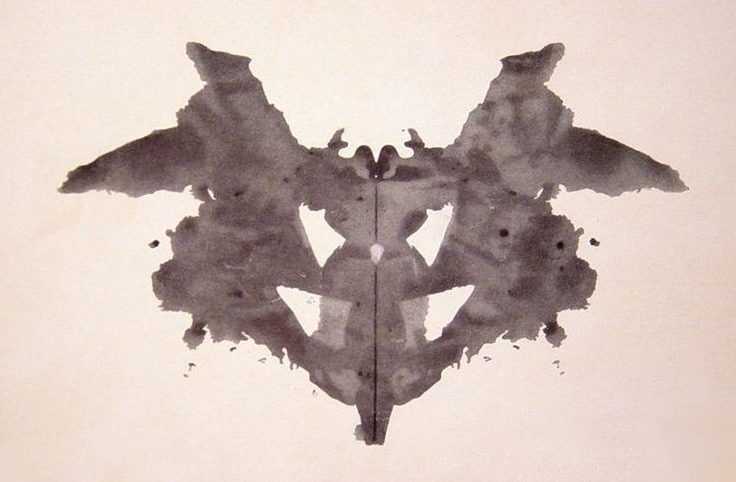
\includegraphics[width=\linewidth]{rorschach_card1.jpg}\par
      {\scriptsize Ռորշախի թեստի առաջին քարտը, 1921}
    \end{column}
    \begin{column}{0.46\textwidth}
      \begin{chatbox}
        Ի՞նչ ես տեսնում այս բծի մեջ։ Գրիր առաջին բանը, որ մտքովդ անցավ
      \end{chatbox}
      \vspace{1mm}
      \alt<3->{%
      \begin{card}[colback=brainpink!25!cardwhite]
        Հազար նման մարդ՝ հազար տարբեր պատասխան։ Լավ ցույց է տալիս անհատականության բարդությունը, բայց \textbf{ստուգել} հնարավոր չէ։
      \end{card}}{%
      \onslide<2->{%
      \begin{card}
        {\blackfont\small Բըրնեթի օրինակները}\par\smallskip
        «Կոկոնից դուրս եկող թիթեռներ»։ Կամ՝ «թերապևտիս պայթած գլուխը, որ չափից շատ հարցեր էր տալիս»։
      \end{card}}}
    \end{column}
  \end{columns}
\end{frame}

% Myth or fact: MBTI
\begin{frame}{Առասպել, թե՞ փաստ \#2}
  \mythorfact{4 տառով MBTI թեստը գիտականորեն հաստատված է}{ԱՌԱՍՊԵԼ}{pinkdark}{%
    \begin{card}[colback=brainpink!25!cardwhite]
      Աշխարհի ամենապոպուլյար թեստերից է ու միլիոնավոր դոլարներ արժե, բայց գիտական հանրությունը այն \textbf{չի ճանաչում}։ Ամենատխուր կիրառությունը՝ ընկերություններում։
    \end{card}}
\end{frame}

% MBTI
\begin{frame}{Մայերս-Բրիգս (MBTI)}
  \begin{columns}[c]
    \begin{column}{0.56\textwidth}
      \begin{itemize}
        \item Myers-Briggs Type \textbf{Indicator} (գրքում՝ Inventory)
        \item Լուրջ տեսք ունի. սանդղակներ, ամենահայտնին՝ էքստրավերտ-ինտրովերտ
        \item<2-> Բայց հիմնված է հին, \textbf{չստուգված ենթադրությունների} վրա, որոնք հավաքել են ոգևորված սիրողներ՝ \textbf{մեկ աղբյուրից}
        \item<3-> Բիզնեսը կառչեց դրանից, ու այսօր այն հարյուր հազարավոր ջատագովներ ունի
      \end{itemize}
    \end{column}
    \begin{column}{0.38\textwidth}
      \centering
      \onslide<4->{%
      \bigemoji[1.6cm]{crystalball}\par\medskip
      \begin{bookquote}
        Բայց հորոսկոպներն էլ ունեն։
      \end{bookquote}}
    \end{column}
  \end{columns}
\end{frame}

% Waiting skeleton + retest
\begin{frame}{Եվ դեռ սպասում ենք}
  \begin{columns}[c]
    \begin{column}{0.4\textwidth}
      \centering
      \begin{meme}[4.4cm]{waiting_skeleton.jpg}
        \memecap[text width=3.6cm]{0.5}{0.9}{MBTI-ի գիտական ապացույցները}
      \end{meme}
    \end{column}
    \begin{column}{0.54\textwidth}
      \onslide<2->{%
      \begin{scienceupdate}
        Լավ թեստը նույն մարդուն երկրորդ անգամ նույն արդյունքը պիտի տա։ MBTI-ն կրկին լրացնողների \textbf{մոտ կեսը} ընդամենը \textbf{5 շաբաթ անց} ստանում է \textbf{ուրիշ} տիպ։ Մեծ հնգյակի թեստերն այս առումով շատ ավելի կայուն են։
      \end{scienceupdate}}
    \end{column}
  \end{columns}
  \onslide<2->{\source{Pittenger, 1993, 2005}}
\end{frame}

% Why companies love it
\begin{frame}{Ինչու է այն սիրում բիզնեսը}
  \begin{columns}[c]
    \begin{column}{0.5\textwidth}
      \begin{itemize}
        \item Պարզ է ու հասկանալի
        \item Աշխատակիցներին բաժանում է հարմար \textbf{խմբերի}, որոնք իբր կանխատեսում են վարքը
        \item<3-> Գոնե տեսականորեն։ Գործնականում չի կարող աշխատել, որովհետև մարդիկ \textbf{բոլորովին էլ այդքան պարզ չեն}
      \end{itemize}
    \end{column}
    \begin{column}{0.46\textwidth}
      \centering
      \begin{tikzpicture}
        \node[pbox=lavender, text width=4.6cm] (i) at (0,1.1) {\emoji{door}\ \textbf{Ինտրովե՞րտ}\\ Թող մենակ աշխատի, մի խանգարեք};
        \node[pbox=peach, text width=4.6cm, visible on=<2->] (e) at (0,-0.9) {\emoji{megaphone}\ \textbf{Էքստրավե՞րտ}\\ Թող զբաղվի գովազդով ու շփումներով. նրանք դա սիրում են};
        \node[visible on=<3->] at (-1.6,-2.55) {\mascot[1.3cm]{confused}};
      \end{tikzpicture}
    \end{column}
  \end{columns}
\end{frame}

% The job application test
\begin{frame}{Աշխատանքի դիմումի թեստ}
  \begin{columns}[c]
    \begin{column}{0.5\textwidth}
      \begin{popup}{դիմում.exe}
        {\blackfont Հարց 7. Սիրու՞մ եք ուրիշների հետ աշխատել}\par\medskip
        $\square$\ Այո, թիմային աշխատանքը իմ ուժն է\par\smallskip
        $\square$\ Կախված է նախագծից\par\smallskip
        \onslide<2->{$\square$\ Ոչ։ Ուրիշները միջատներ են, որոնք կան միայն ճզմվելու համար}
      \end{popup}
    \end{column}
    \begin{column}{0.44\textwidth}
      \onslide<3->{%
      \begin{itemize}
        \item Թեստն աշխատում է, եթե դիմողը 100\% անկեղծ է ու գրեթե նույնքան միամիտ
        \item Շատերը «ապահով» են պատասխանում, ու արդյունքը \textbf{անիմաստ} է դառնում
      \end{itemize}}
      \onslide<4->{%
      \begin{poll}
        Ձեռք բարձրացրու, եթե թեստին երբևէ պատասխանել ես այնպես, ինչպես \textbf{«պետք է»}
      \end{poll}}
    \end{column}
  \end{columns}
\end{frame}

% Section end
\begin{frame}{Թեստերը՝ մեկ էջում}
  \begin{columns}[T]
    \begin{column}{0.47\textwidth}
      \begin{card}[colback=mint!35!cardwhite]
        \emoji[1.3em]{check}\ {\blackfont Մեծ հնգյակ}\par\smallskip
        Լավագույնն է, ինչ ունենք. կայուն գծեր, կապ ուղեղի ու գեների հետ։ Բայց ոչ ամբողջական, ու չգիտենք՝ որն է պատճառը, որը՝ հետևանքը
      \end{card}
    \end{column}
    \begin{column}{0.47\textwidth}
      \begin{card}[colback=brainpink!25!cardwhite]
        \emoji[1.3em]{cross}\ {\blackfont MBTI ու օնլայն թեստեր}\par\smallskip
        Զվարճալի են, բայց գիտական չեն։ Ու մի որոշիր աշխատակցի ճակատագիրը չորս տառով
      \end{card}
    \end{column}
  \end{columns}
  \vspace{3mm}
  \onslide<2->{%
  \begin{bookquote}
    Անհատականության թեստերն ավելի օգտակար կլինեին, եթե մեր անհատականությունները չխանգարեին։
  \end{bookquote}}
\end{frame}

% ---------------------------------------------------------------- break
\begin{frame}[plain]
  \begin{tikzpicture}[remember picture, overlay]
    \fill[butter!60!cream] (current page.south west) rectangle (current page.north east);
    \node at ([yshift=8mm]current page.center) {\mascot[4cm]{sleepy}};
    \node[anchor=north, font=\titlefont\fontsize{30}{32}\selectfont, text=plum] at ([yshift=-17mm]current page.center) {Ընդմիջում};
    \node[anchor=north, font=\mediumfont\large, text=plum] at ([yshift=-31mm]current page.center)
      {5 րոպե \emoji{coffee}\quad Կանգնիր, ձգվիր, ջուր խմիր};
  \end{tikzpicture}
\end{frame}
